\section{Gaussian Processes}
\begin{frame}{Background}
    \begin{block}{Function Approximation}
        $\mathrm{f}:x \mapsto y$
    \end{block}
    \pause
    \begin{block}{Parametric Models: Pros}
        Easy to interpret
    \end{block}
    \begin{block}{Parametric Models: Cons}
        \begin{itemize}
            \item Simpler models lack expressive power
            \item Complex models require lots of data
            \item Predictions are dependent on the model
            \item Representation of uncertainty in the input space
            \end{itemize}
    \end{block}
\end{frame}

\begin{frame}{Linear Regression Model}
    $y = x+0.005x^2+ \epsilon$, $x \in [1,10] \cup [21,25]$,  $\epsilon \sim \mathcal{N}(0,10)$ 
    \begin{figure}
        \centering
        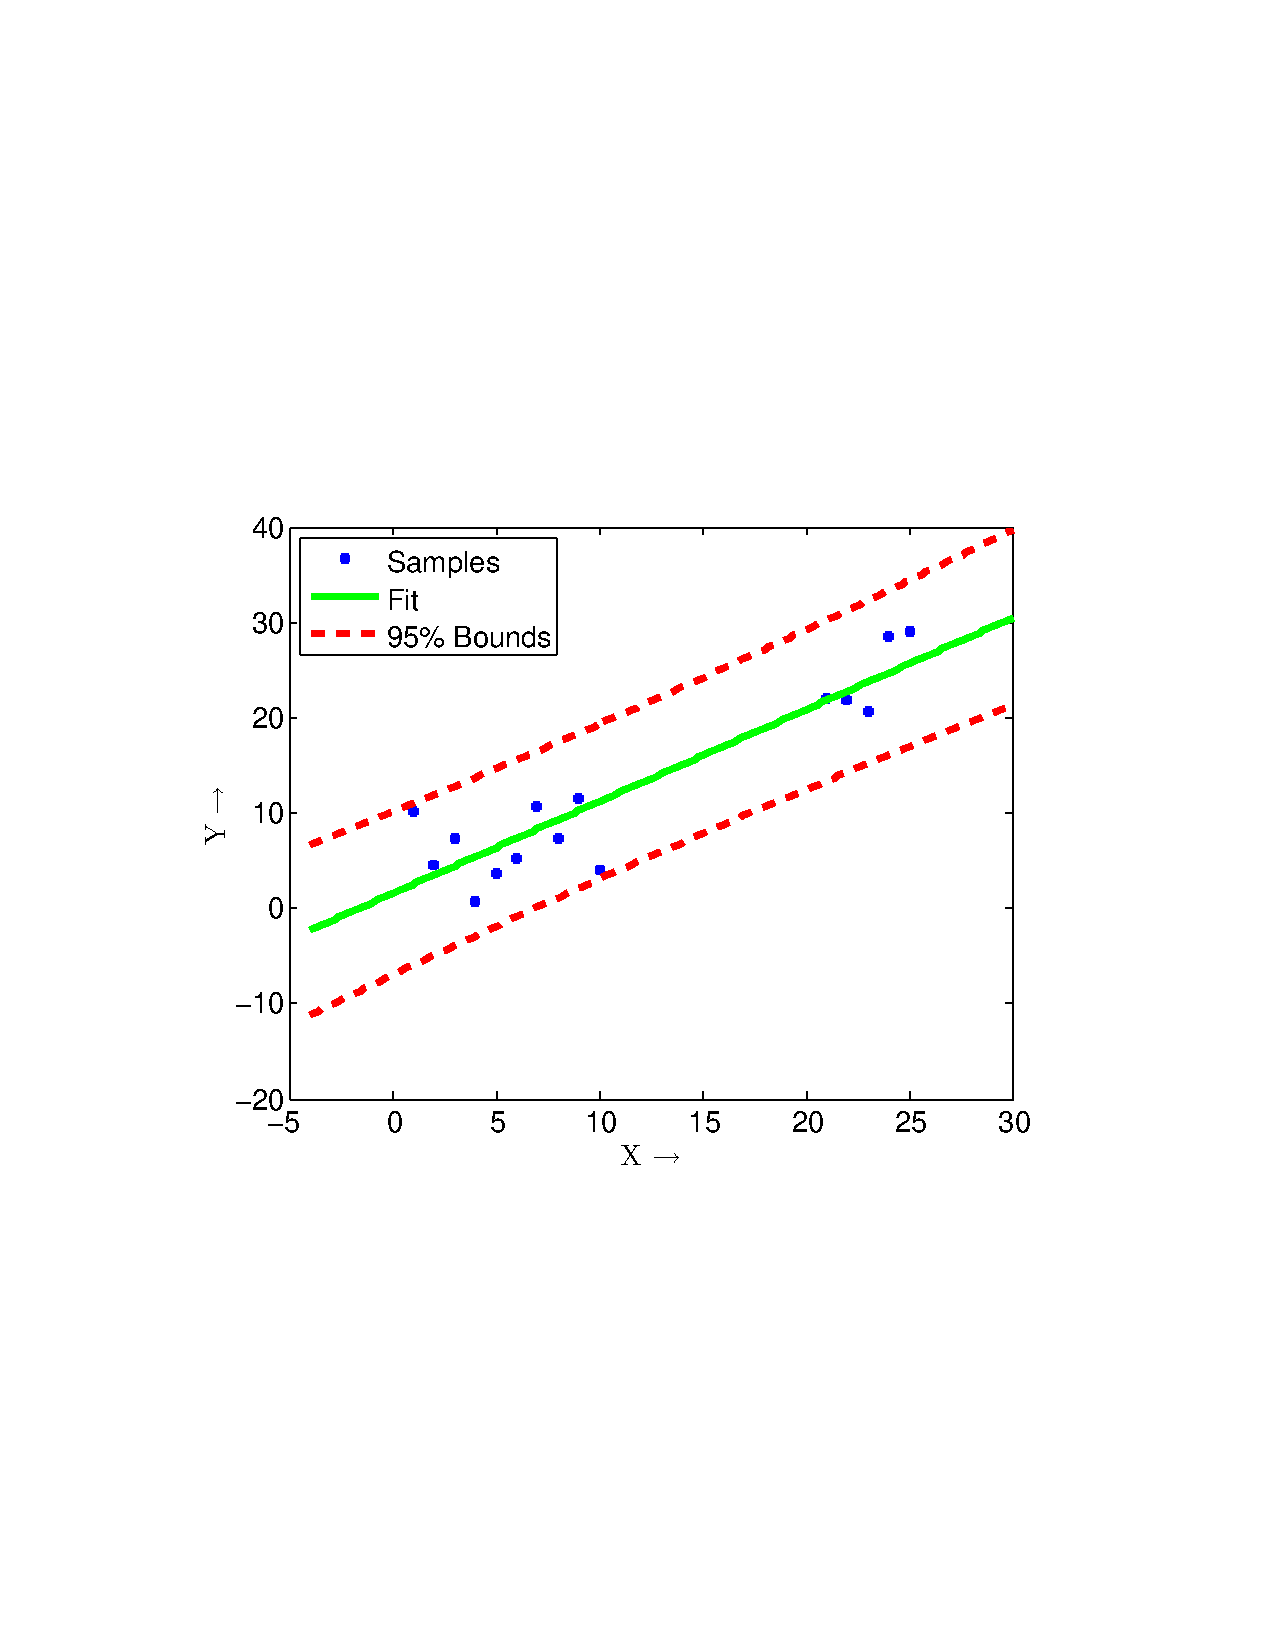
\includegraphics[width=0.5\linewidth,trim=30mm 80mm 40mm 70mm,clip]{figures/linear_fit}
        \caption{Linear Regression yields the model $y=mx+c$ with $m = 0.9644$ and $c = 1.5891$ }
    \end{figure}
\end{frame}

\begin{frame}{Quadratic Regression Model}
$y = x+0.005x^2+ \epsilon$, $x \in [1,10] \cup [21,25]$,  $\epsilon \sim \mathcal{N}(0,10)$
\begin{figure}
    \centering
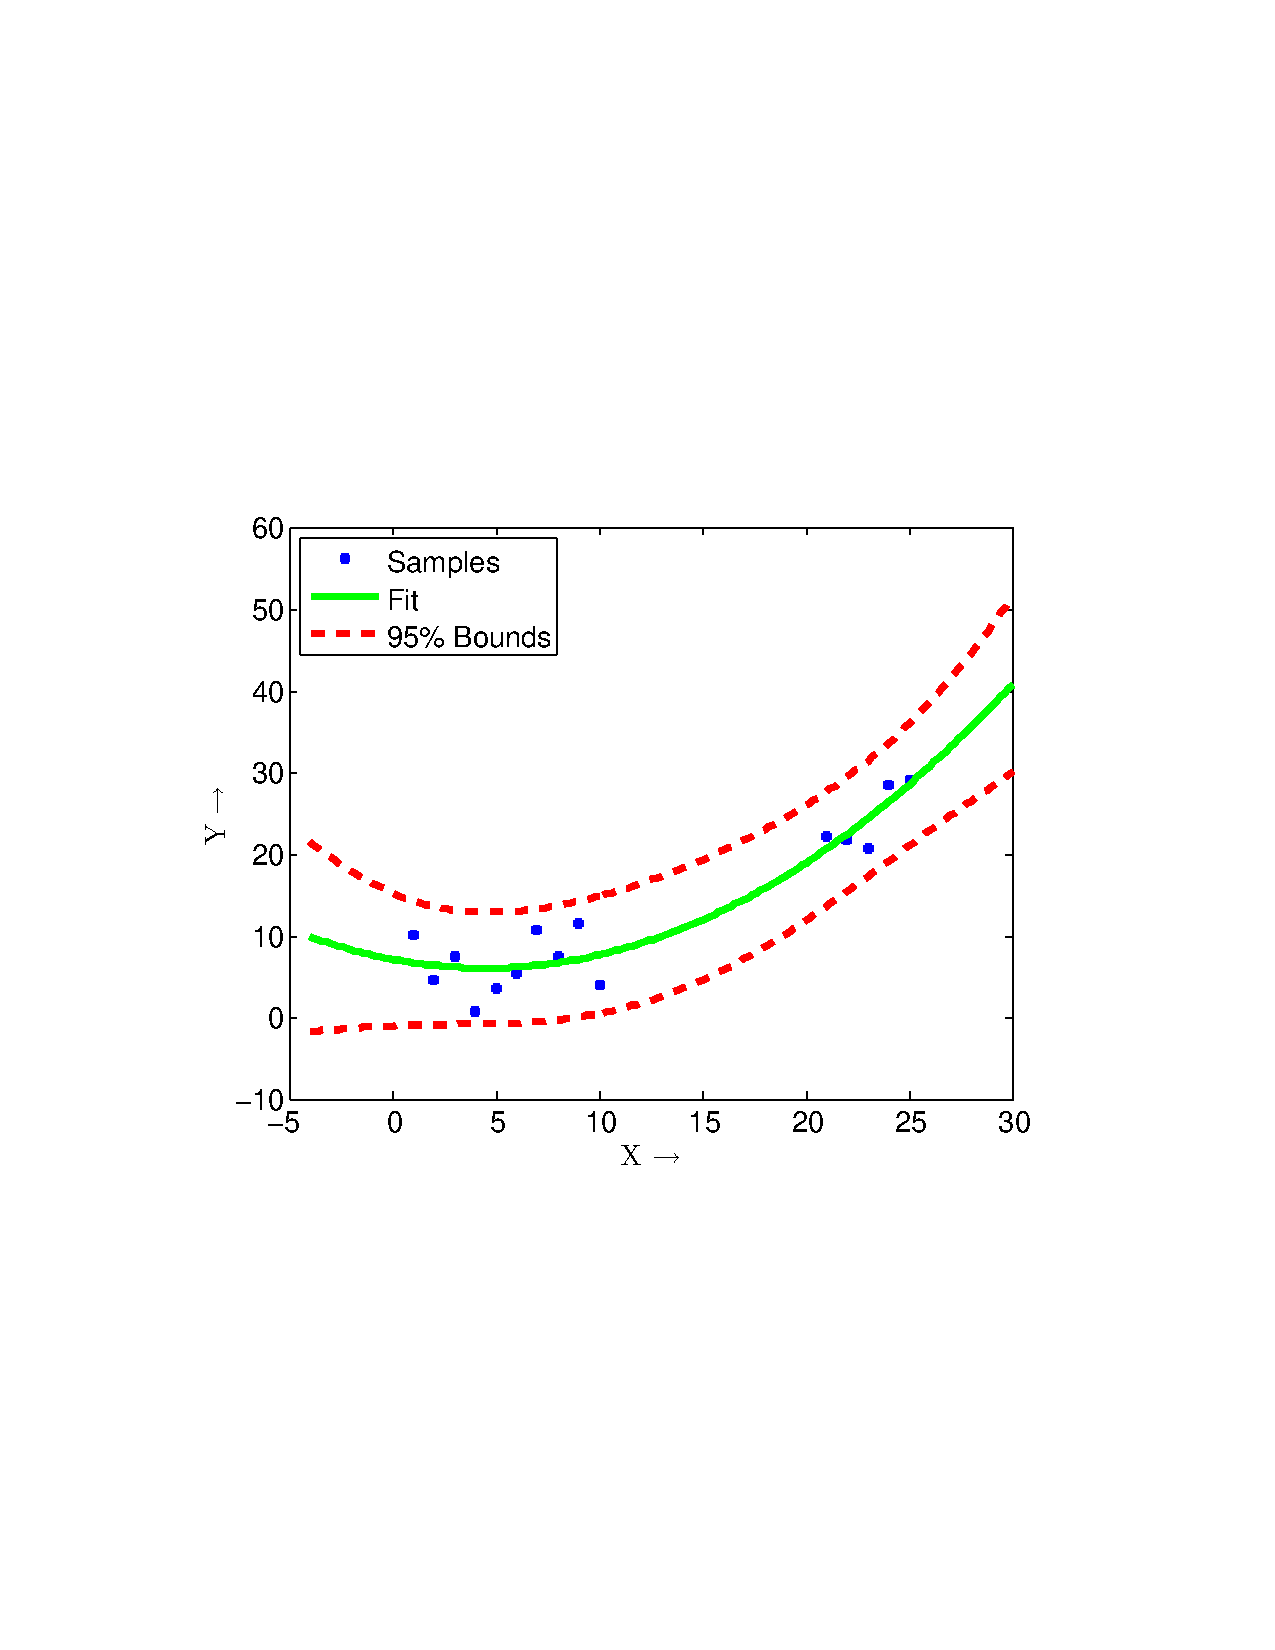
\includegraphics[width=0.5\linewidth,trim=30mm 80mm 40mm 70mm,clip]{figures/quadratic_fit}
\caption{ Quadratic model yields the model $y = ax^2+bx+c$ with $a = 0.0534$, $b = -0.04781$ and $c = 7.1231$}
\end{figure}

\end{frame}

\begin{frame}{Bayesian Linear Regression}
$y = x+0.005x^2+ \epsilon$, $x \in [1,10] \cup [21,25]$,  $\epsilon \sim \mathcal{N}(0,10)$ 
\begin{figure}
\centering
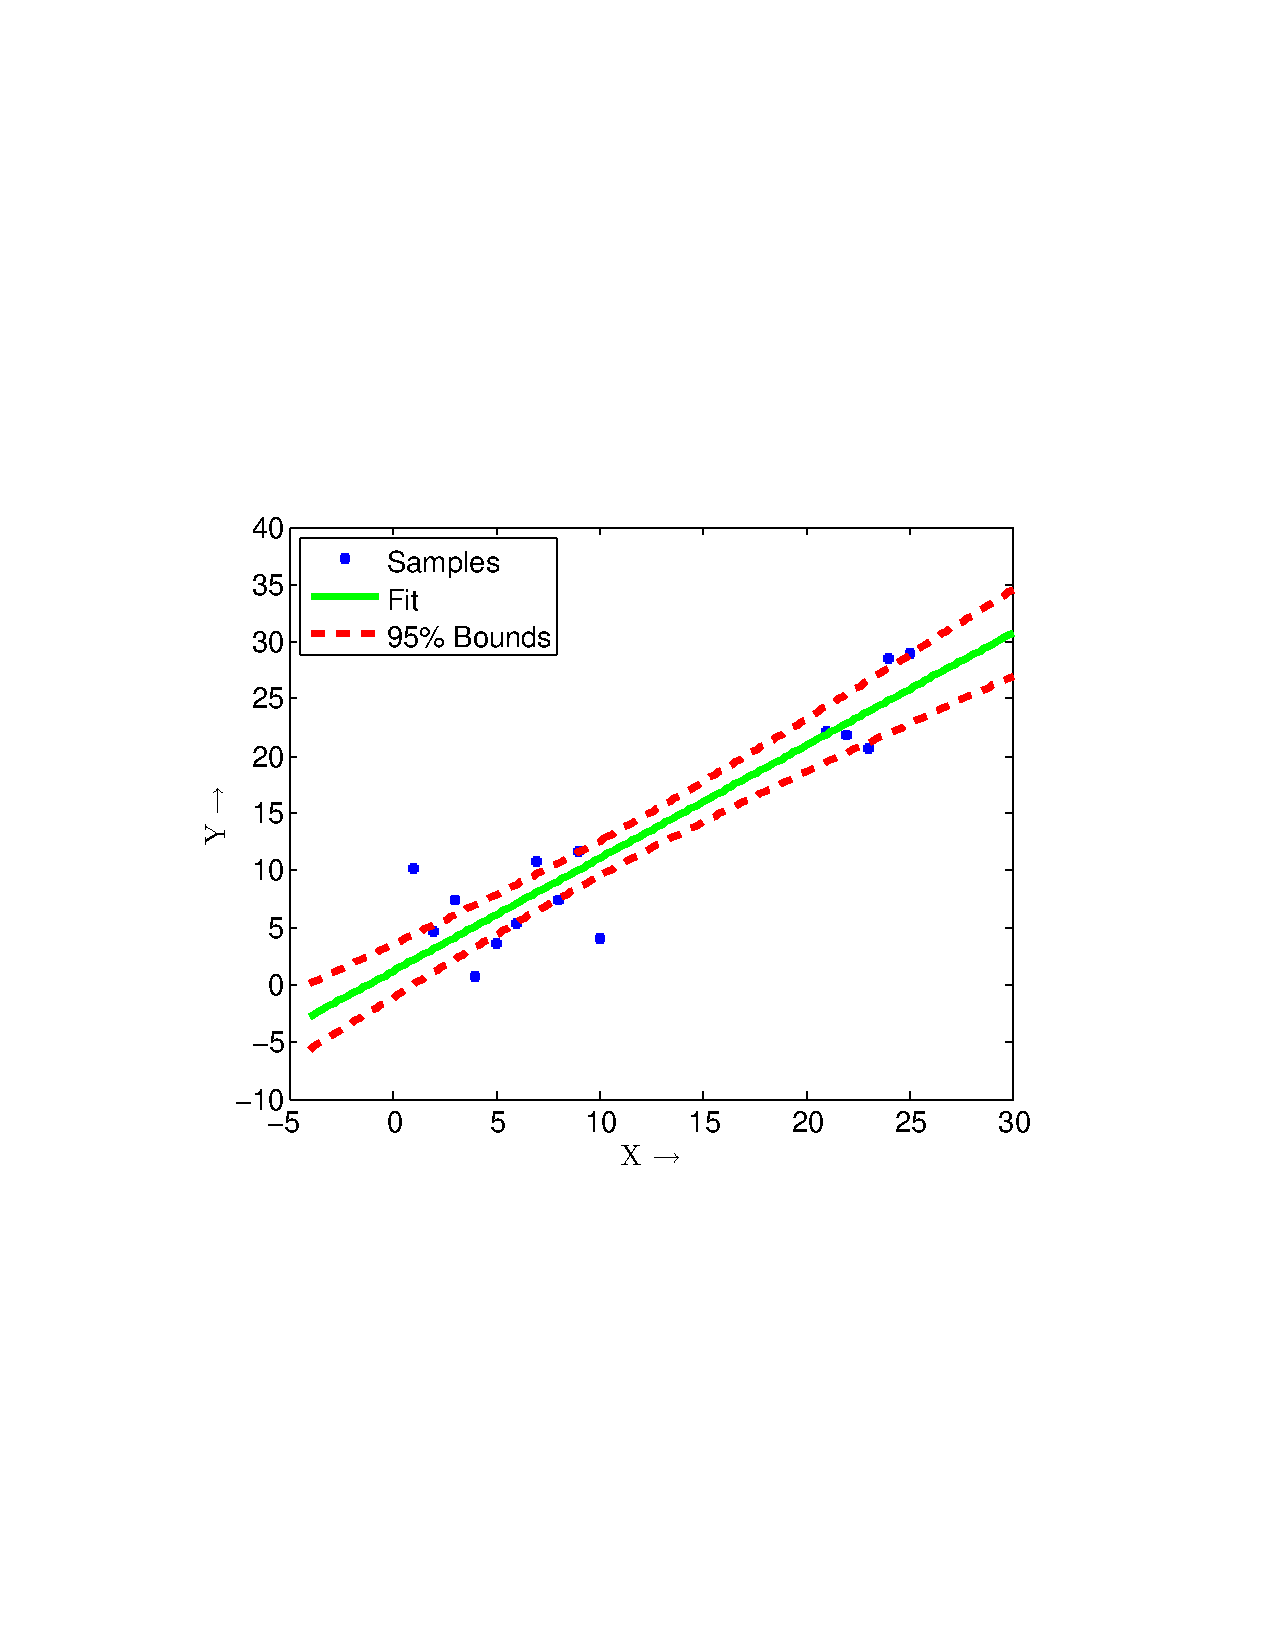
\includegraphics[width=0.5\linewidth,trim=30mm 80mm 40mm 70mm,clip]{figures/bayesian_linear_fit}
\caption{ Bayesian Regression fit uses a zero mean Gaussian observation noise with  variance $10$ and a zero mean Gaussian with diagonal variance $5$ prior on slope and intercept. The estimation process results in a mean parameter estimate of $0.9867$ slope and $1.1797$ intercept.}
\end{figure}
\end{frame}

\begin{frame}{Gaussian Process}
    \begin{block}{Definition}
        Gaussian Process is a collection of random variables, any finite number
        of which are joint Gaussian distribution. \\
$f(x) \sim \mathbb{GP}(m(x),k(x,x^1))$
    \end{block}
    \begin{itemize}
        \item Generalization from mean vector and covariance matrix
        \item Indexed by $x$
        \item At every value of $x$, we have an associated random variable
        \end{itemize}


\end{frame}

\begin{frame}{Visualizing Gaussian Process}
$f(x) \sim \mathbb{GP}(m(x),k(x,x^1))$ \\
$m(x) = \frac{1}{4}x^2,$ and $k(x,x^1) = \exp{(-\frac{1}{2}(x-x^1)^2)}$\\
Let's sample at $n$ different locations\\
$\mu(x_i) = \frac{1}{4}x_i^2,$ and $\Sigma_{ij}(x_i,x_j) =
\exp{(-\frac{1}{2}(x_i-x_j)^2)}$, $i,j \in [1,...,n]$
\begin{figure}
\centering
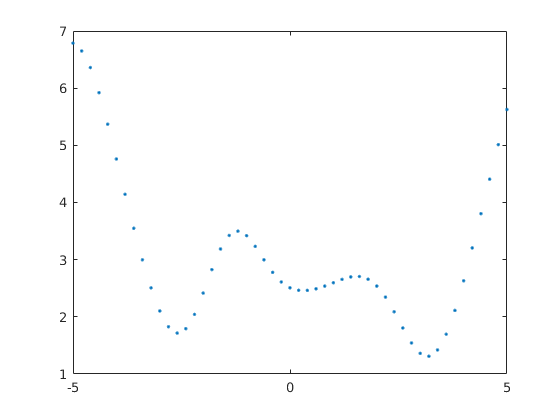
\includegraphics[width=0.5\linewidth]{figures/converted_sampling_gp}
\end{figure}
\end{frame}

\begin{frame}{Posterior Gaussian Process}
$f(x): x \mapsto y$. 
\begin{itemize}
    \item Input: Ground truth data  from $(\mathbf{x},\mathbf{f(x)})$ from $n$ observations
\item Output: Output $f_*$ for a novel input $x_*$, $p(y_*|x_*)$. 
\item Measurement Process: $y = f(x)+\epsilon $, $\epsilon \sim \mathcal{N}(0,\sigma^2)$
\end{itemize}
Joint Distribution:
\begin{align}
    \begin{bmatrix}
        f \\
        f_*
    \end{bmatrix}& \sim
    \mathcal{N}\left(
    \begin{bmatrix}
        \mu\\
        \mu_*
    \end{bmatrix}, 
    \begin{bmatrix}
        \Sigma & \Sigma_* \\
        \Sigma_*^T & \Sigma_{**}
    \end{bmatrix}
    \right)
\end{align}
Marginalization:
\begin{align}
    f_*|f \sim
    \mathcal{N}(u_*+\Sigma_*^T\Sigma^{-1}(f-\mu),\Sigma_{**}-\Sigma_*^T\Sigma^{-1}\Sigma_*)
\end{align}

\end{frame}

\begin{frame}{Posterior Gaussian Process}
 Posterior Process:
\begin{align}
    \mathbf{f}|\mathcal{D} \sim & \mathbb{GP}(m_D,k_D) \nonumber\\
    & m_D(x) = m(x) + \Sigma(X,x)^T\Sigma^{-1}(f-m) \nonumber\\
    & k_D(x,x^1) = k(x,x^1) - \Sigma(X,x)^T\Sigma^{-1}\Sigma(X,x^1)
\end{align}

Observation Noise:
\begin{align}
    y & \sim \mathbb{GP} (m,k+\sigma_n^2\delta_{ii^1})
\end{align}
\end{frame}

\begin{frame}{Training Hyper-parameters}
    Parameterizing GP Priors \\
    $m(x) = ax^2+bx+c$, and $k(x,x^1) = \sigma_y^2\exp{(-\frac{(x-x^1)^2}{2l^2})}+\sigma^2_n\delta_{ii^1}$ \\
    Hyperparameters: $\theta = \{a,b,c,\sigma_y,\sigma_n,l\}$ \\
    Fitting:
    \begin{align}
        L &= \log{p(y|x,\theta)} \nonumber\\
          &= -\frac{1}{2}\log|\Sigma| - \frac{1}{2} (y-\mu)^T\Sigma^{-1}(y-\mu) -
        \frac{n}{2}\log{2\pi}
    \end{align}
    Estimation:
    \begin{align}
        \frac{\partial L}{\partial \theta_m}& = -(y-\mu)^T\Sigma^{-1}\frac{\partial m}{\partial \theta_m} \nonumber \\
        \frac{\partial L}{\partial \theta_k}& = \frac{1}{2} trace(\Sigma^{-1}\frac{\partial \Sigma}{\partial \theta_k})+\frac{1}{2}(y-\mu)^T\frac{\partial \Sigma}{\partial \theta_k}\Sigma^{-1}\frac{\partial \Sigma}{\partial \theta_k}(y-\mu)
    \end{align}
Non-parametric does not mean no parameters. Parametric models can through
    away data once parameters are tuned.
\end{frame}

\begin{frame}{Gaussian Process Regression}
$y = x+0.005x^2+ \epsilon$, $x \in [1,10] \cup [21,25]$,  $\epsilon \sim \mathcal{N}(0,10)$ 
\begin{figure}
\centering
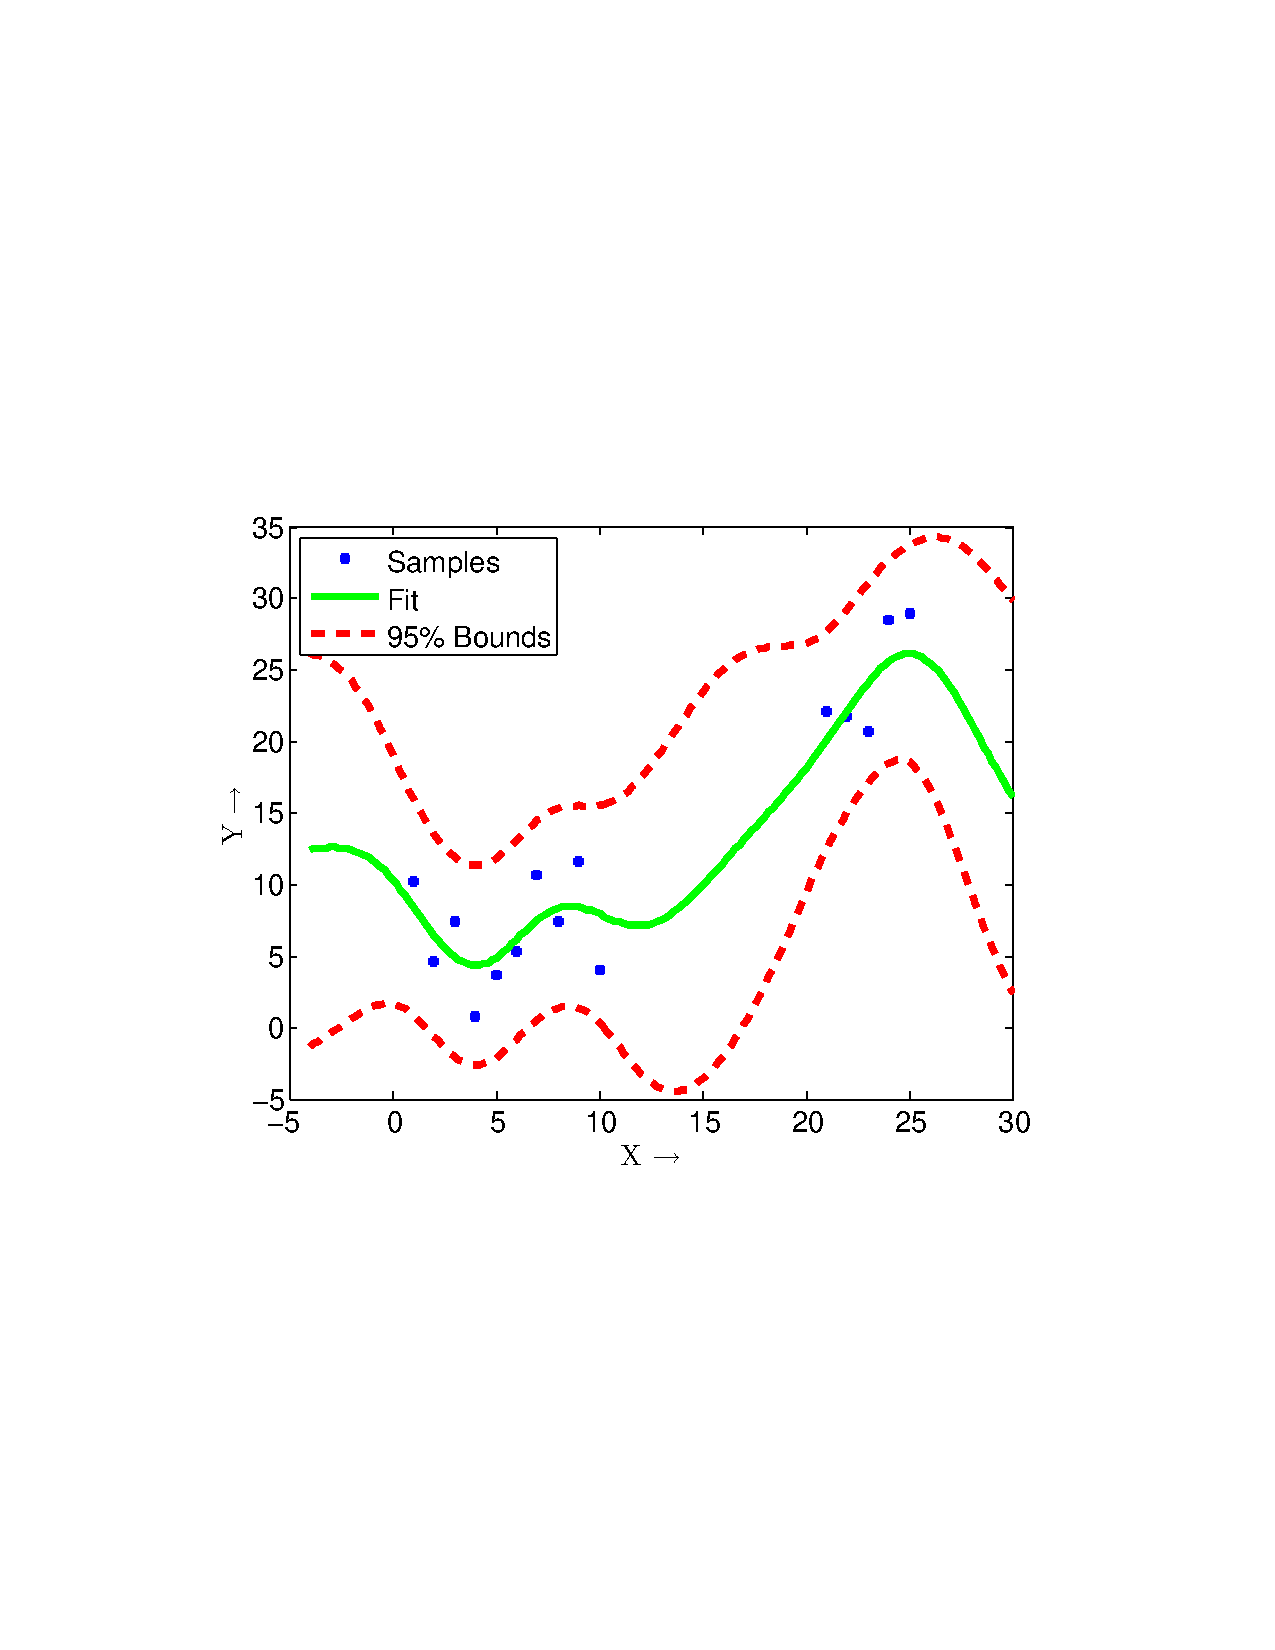
\includegraphics[width=0.5\linewidth,trim=30mm 80mm 40mm 70mm,clip]{figures/gpml_fit}
\caption{ GPR with constant mean function, Gaussian likelihood and Squared Exponential covariance function}
\end{figure}
\end{frame}


